\chapter{Reconstructor}
\label{sec:reconst} 

The reconstructor associates all available target reports to unique targets, each identifed by a \textbf{U}nique \textbf{T}arget \textbf{N}umber (\textbf{UTN}). For each of the targets, reference trajectories ("optimal" position estimates akin to system track updates) are calculated and written to the database. \\

Reference trajectories are calculated based on available sensors and System Trackers, as selected by the user. \\

2 different reconstructors exist, but the advanced reference trajection calculation feature (Probabilistic + IMM Reconstructor) is only available under a commercial professional license. In the free license, a basic reconstructor (Scoring + UMKalman) is available. Please refer to \nameref{sec:ui_configure_licenses} for licensing information. \\

\begin{itemize}  
   \item Basic: Scoring + UMKalman
   \begin{itemize}  
   \item Included in free version
   \item Association based on secondary attributes and simple, configurable distance scoring
   \item Position estimation using Linear Uniform Motion Kalman filter
   \end{itemize}  
   \item Advanced: Probabilistic + IMM
   \begin{itemize}  
   \item Requires commercial professional license
   \item Association based on secondary attributes and self-adaptive probabilistic thresholds
   \item Uses Radar bias estimation \& correction, ADS-B geometric altitude for slant range correction, accuracy -re-estimation and scaling, ADS-B verification, ...
   \item Position estimation using Interacting Multiple Models (IMM) filter, with a Rauch-Tung-Striebel (RTS) smoother
   \end{itemize}
\end{itemize}  

\section{Workflow}

For optimal performance, the processing of the target reports and reconstruction is time-sliced. In (commonly) 15 minute intervals, all target reports are loaded, associated to UTNs, references are calculated and written to the database, after which the next time-slice is loaded. \\

In the 'Probabilistic + IMM' reconstructor, each data slice is processed multiple times, to re-estimate correctable bias' as well as rescale target report accuracies. \\

For each processed slice, the following general steps are performed:

\begin{itemize}
\item Load all target reports for the current time-slice
\item Remove all target reports / calculated information for the previous time-slice
\item Load all target reports, per data source
\item Associate target reports to UTNs
   \begin{itemize}  
   \item If possible, associate by matching reliable secondary attribute
    \begin{itemize}  
    \item Mode S Address, Mode S Identification, Reliable Track Number
    \end{itemize}
   \item Otherwise, associate by matching Mode A/C and position
    \begin{itemize}  
    \item Ignoring conspicuity codes
    \end{itemize}    
   \item Otherwise, associate by position only
   \end{itemize}
\item Self-associate new targets (find matching UTNs created by the same target)
\item Retry-Associate target reports
\item Compute references
\item Calculate statistics based on references
\item Write references \& associations
\end{itemize}
\ \\

\section{Dialog}

\subsection{Common}

\begin{figure}[H]
    \center
      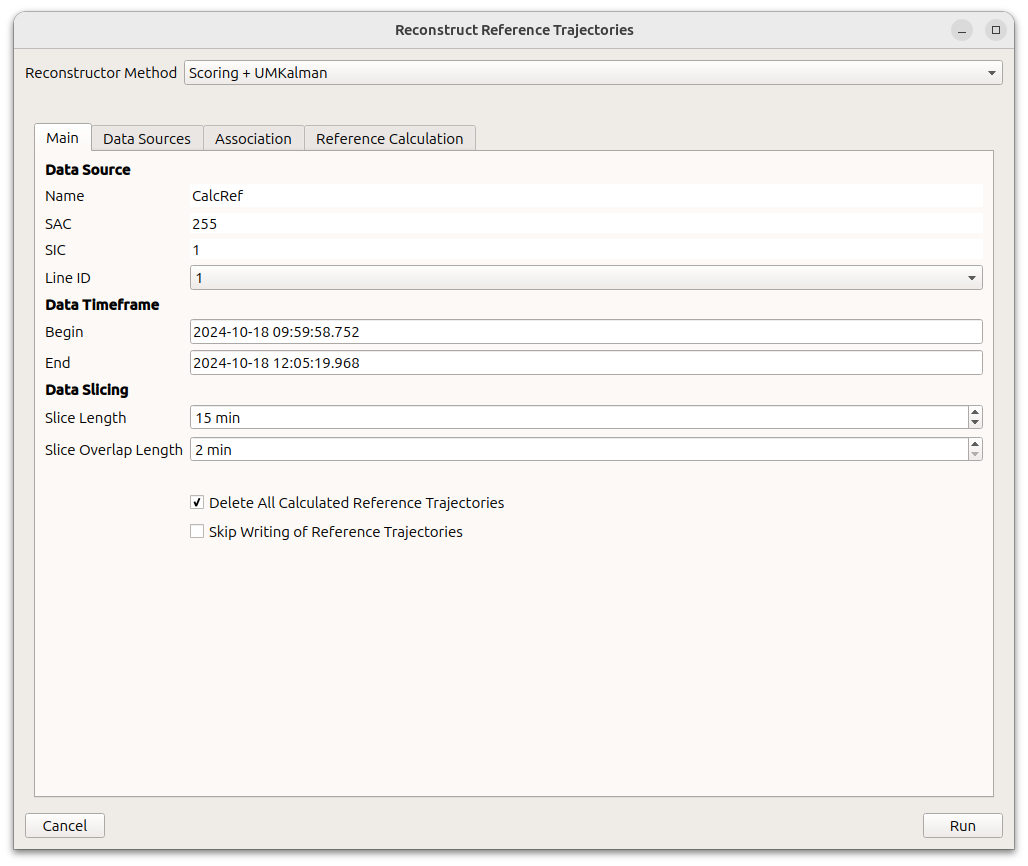
\includegraphics[width=16cm]{figures/dialog_main.png}
    \caption{Calculate References Main}
\end{figure}

In the main tab, the following parameters can be set:

\begin{itemize}
\item Data Source: Data source to be created for calculated references
    \begin{itemize}
    \item Name, SAC, SIC: Data source parameters
    \item Line ID: Line ID to be used
    \end{itemize}
\item Data Timeframe: Time window of data to be processed
    \begin{itemize}
    \item Begin / End timestamps
    \end{itemize}
\item Data Slicing: Time slice sizes
    \begin{itemize}
    \item Slice Length: Duration of a time slice
    \item Slice Overlap Length: Duration of an overlap region to "glue" slices together
    \end{itemize}
\item Delete All Calculated Reference Trajectories: If active, all previous calculated references are deleted
\item Skip Writing of Reference Trajectories: If active, calculated references are not written into the database, only the associations
\end{itemize}
\ \\

\begin{figure}[H]
    \center
      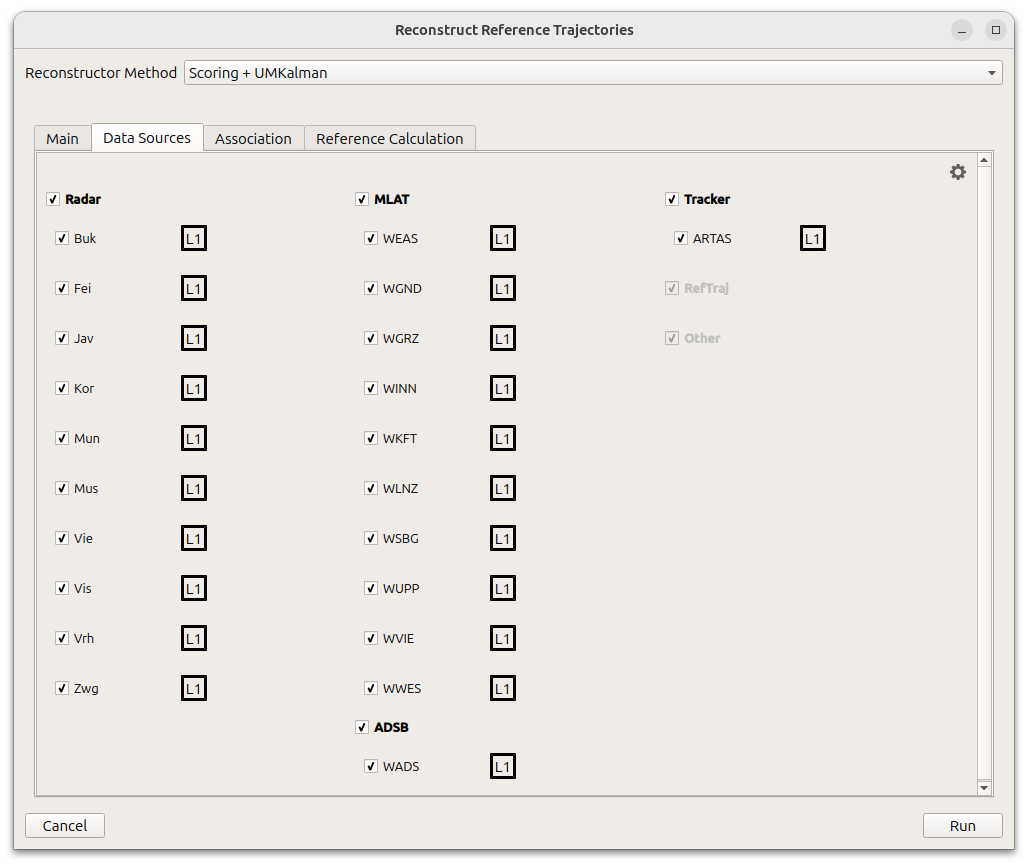
\includegraphics[width=16cm]{figures/dialog_data_sources.png}
    \caption{Calculate References Data Sources}
\end{figure}

In this tab, the data sources to contribute to the calculated references can be selected. \\

Please \textbf{note} that de-selected data sources are still associated, but only their target report positions do not contribute to the references.

\subsection{Scoring + UMKalman Parameters}

\begin{figure}[H]
    \center
      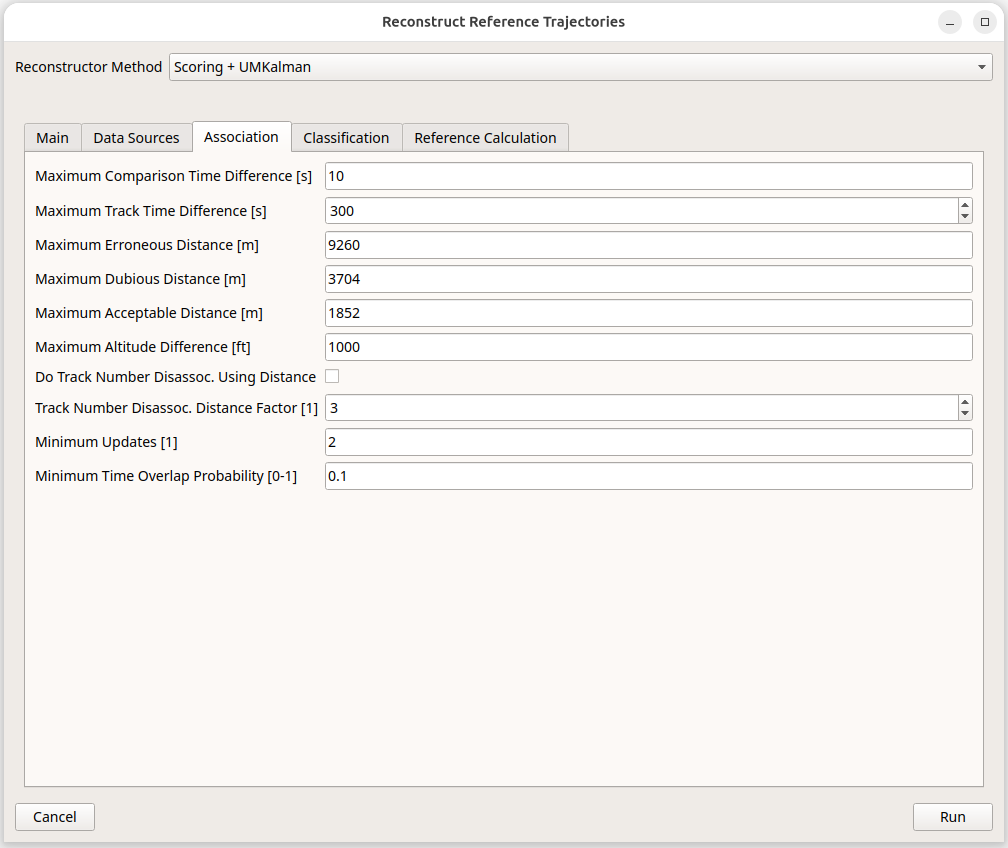
\includegraphics[width=16cm]{figures/dialog_scorum_assoc.png}
    \caption{Scoring + UMKalman Association Parameters}
\end{figure}

\begin{table}[H]
  \center
  \begin{tabularx}{\textwidth}{ | l | l | X |}
    \hline
    \textbf{Parameter} & \textbf{Default} &  \textbf{Description} \\ \hline
    Maximum Comparison Time Difference [s] & 15 & Maximum time delta for any code/position comparison \\ \hline
    Maximum Quit Distance [m] & 18520 & Target/target association \\ \hline
    Maximum Dubious Distance [m] & 5556 & Target/target association \\ \hline
    Maximum Acceptable Distance [m] & 1852 & Target/target association \\ \hline
    Maximum Altitude Difference [ft] & 300 & Maximum altitude difference \\ \hline
    Do Track Number Disassoc. Using Distance & false & Whether to disassociated track numbers from targets based on position \\ \hline
    Track Number Disassoc. Distance Factor [1] & 3 & Maximum number of standard deviations distance \\ \hline
    Minimum Updates [1] & 2 & Target/target association \\ \hline
    Minimum Time Overlap Probability [0-1] & 0.1 & Target/target association \\ \hline
  \end{tabularx}
\end{table}

\begin{figure}[H]
    \center
      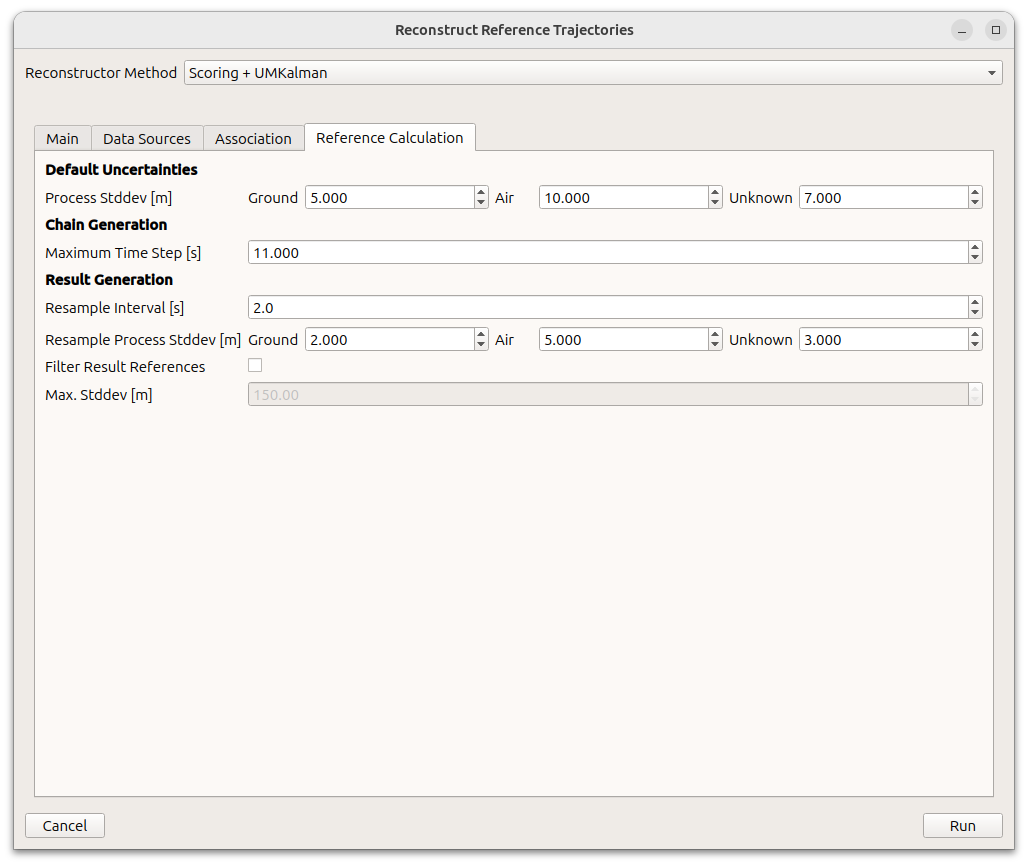
\includegraphics[width=16cm]{figures/dialog_ref_calc.png}
    \caption{Scoring + UMKalman Reconstruction Parameters}
\end{figure}

\begin{table}[H]
  \center
  \begin{tabularx}{\textwidth}{ | l | l | X |}
    \hline
    \textbf{Parameter} & \textbf{Default} &  \textbf{Description} \\ \hline
    Process Stddev [m] Ground & 3 & Process noise for ground targets \\ \hline
    Process Stddev [m] Air & 10 & Process noise for FL400 targets \\ \hline
    Process Stddev [m] Unknown & 7 & Process noise for targets w/o altitude \\ \hline
    Maximum Time Step [s] & 11 & Re-init reference if no update available within given time \\ \hline
    Resample Process Stddev [m] Ground & 2 & Resampling process noise for ground targets \\ \hline
    Resample Process Stddev [m] Air & 5 & Resampling process noise for FL400 targets \\ \hline
    Resample Process Stddev [m] Unknown & 3 & Resampling process noise for targets w/o altitude \\ \hline    
    Filter Result References& false & Whether to filter written reference trajectory updates based on maximum position standard deviation \\ \hline
    Max. Stddev [m] & 150 & Maximum position standard deviation \\ \hline
  \end{tabularx}
\end{table}


\subsection{Probabilistic + IMM Parameters}

\begin{figure}[H]
    \center
      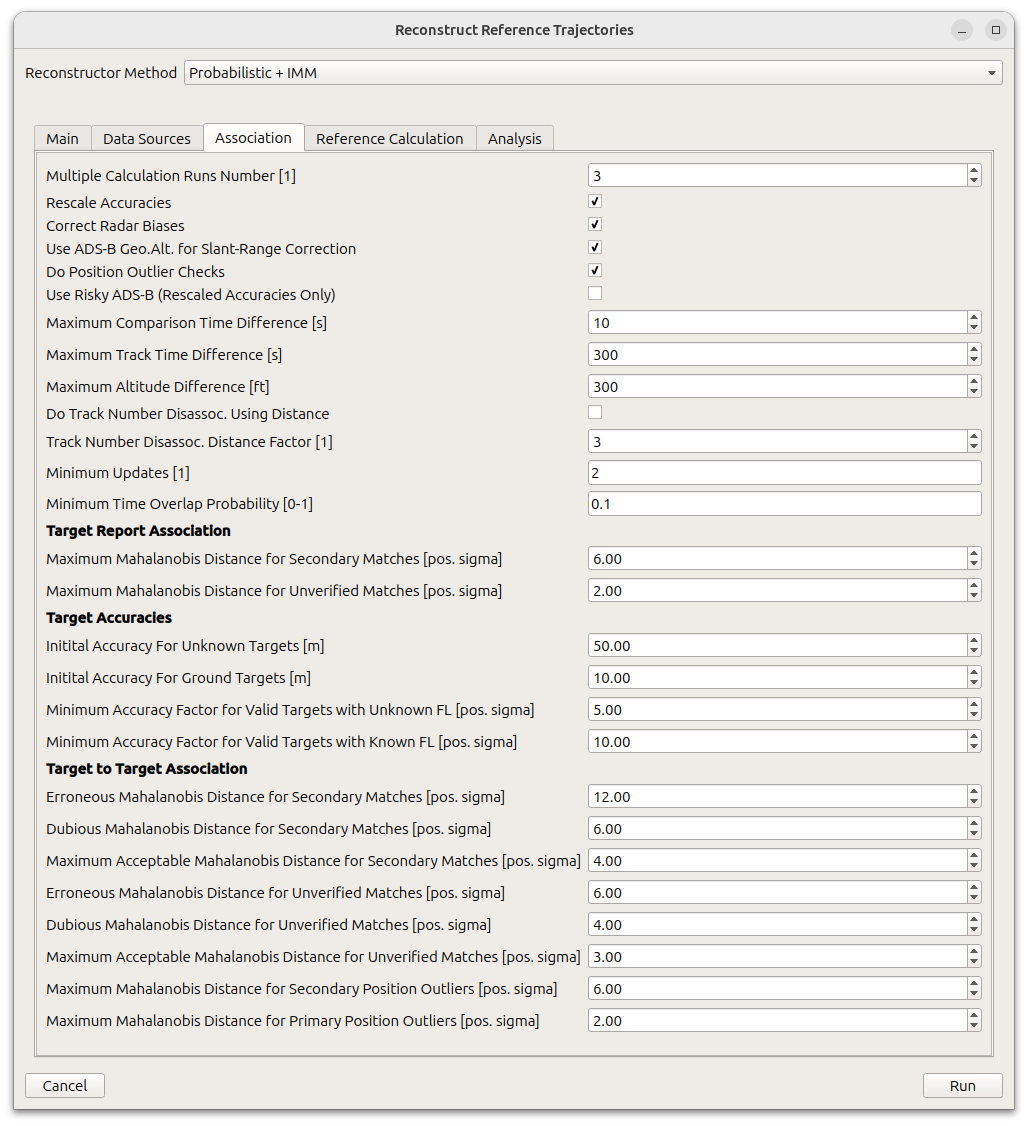
\includegraphics[width=16cm]{figures/dialog_probimm_assoc.png}
    \caption{Probabilistic + IMM Association Parameters}
\end{figure}

\begin{figure}[H]
    \center
      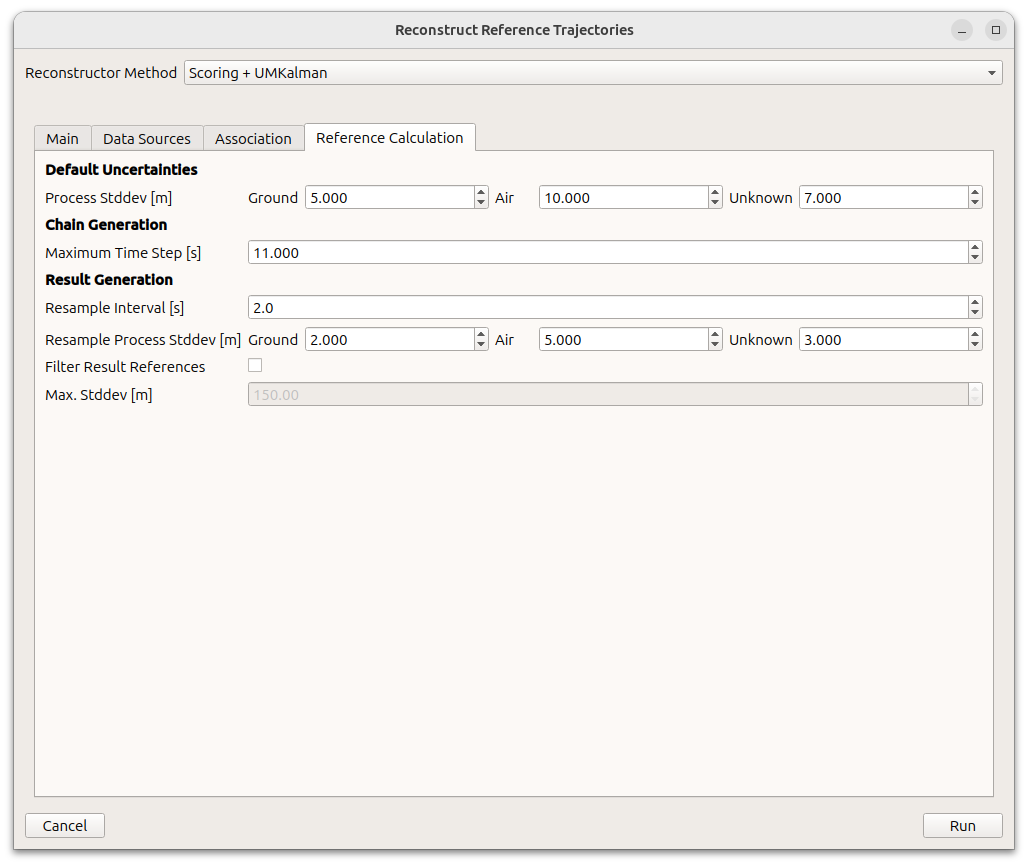
\includegraphics[width=16cm]{figures/dialog_ref_calc.png}
    \caption{Probabilistic + IMM Reconstruction Parameters}
\end{figure}

\begin{figure}[H]
    \center
      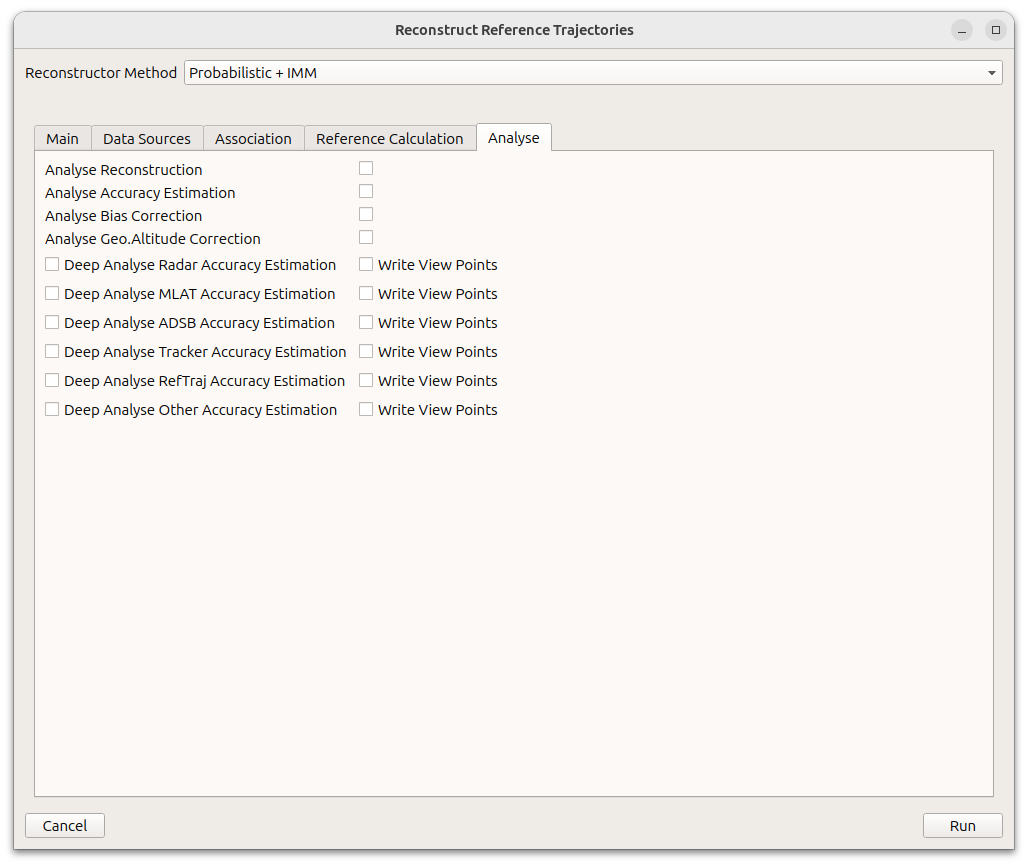
\includegraphics[width=16cm]{figures/dialog_probimm_analyse.png}
    \caption{Probabilistic + IMM Analysis Parameters}
\end{figure}


\section{Calculate Unique Targets}


The other parameters are discussed in following sub-sections.

\subsubsection{Reference/Tracker UTN Creation}

Track/Track Association Parameters:
\begin{table}[H]
  \center
  \begin{tabularx}{\textwidth}{ | X | l | X |}
    \hline
    \textbf{Parameter} & \textbf{Default} &  \textbf{Used In} \\ \hline
    Maximum Comparison Time Difference [s] & 15.0 & All (maximum time delta for any code/position comparison) \\ \hline

    Maximum Altitude Difference [ft] & 300 & Target/target association \\ \hline

    Max Speed [kts] & 100000 & Dubious target detection \\ \hline
    Maximum Continuation Time Difference [s] & 30 & Track continuation \\ \hline
    Maximum Acceptable Continuation Distance [m] & 1852 & Track continuation \\ \hline
  \end{tabularx}
\end{table}
\ \\

The following steps are performed for each Reference/Tracker data source:
\begin{itemize}
\item Per-source target creation
\begin{itemize}
\item Create new list of targets based on
\begin{itemize}
\item Track number
\item Mode S address
\item Mode A/C, time difference, position difference (track continuation)
\end{itemize}
\item Find dubious targets (dubious target detection)
\item Clean dubious targets (if configured)
\end{itemize}
\begin{itemize}
\item Per-source target to common target association (target/target association)
\item Score-based approach
\item Associates new per-source targets to existing targets based on
\begin{itemize}
\item Mode S address
\item Time overlap
\item Mode A code(s) similiarity (only if minimum time overlap is given)
\item Mode C code(s) similiarity (only if Mode A similiarity is given)
\item Position similiarity (only if Mode A/C similiarity is given)
\end{itemize}
\end{itemize}
\end{itemize}
\ \\

After creating targets for all Reference/Tracker data sources:
\begin{itemize}
\item Find dubious targets
\item Clean dubious targets (if configured)
\item Mark/comment dubious targets (if configured)
\end{itemize}
\ \\

The exact method discussion will be added at a later time, since the algorithms will be improved to include position accuracy information (error standard deviation etc.) in the near future. \\

After these steps, for each target which can be created by the simple score-based association method will be used to additionally associate sensor target reports (non Reference/Tracker based target reports), as discussed in the next section.

\subsubsection{Sensor UTN Creation}



The following steps are performed for each sensor data source:
\begin{itemize}
\item Find possible target in existing target list based on
\begin{itemize}
\item Mode S address
\item Mode A code similiarity (if present)
\item Mode C code similiarity (if present)
\item Position similiarity
\end{itemize}
\item If a matching target is found, the best match is used for association
\item If no matching target is found
\begin{itemize}
\item If the target report has Mode S address, a new target is created
\item Otherwise no association is made
\end{itemize}
\end{itemize}
\ \\

\subsubsection{Dubious Targets}

The dubious target check is solely based on a simple maximum speed given all associated Reference/Tracker target reports. It should be used to detect/mark possibly wrong associations, to investigate such targets later and, if possible, resolve such issues using different parameter values. \\

Please note that in a special case where target reports from difference Reference/Tracker source are very close in time this check can generate a large number of false positives and should be disabled. For this reason the default value was set to a disproportionately high value.

\subsubsection{Discussion}

The user should be aware that, while this association feature is quite an improvement over the previous method, it is still somewhat limited. It strongly depends on the correctness of Mode S addresses, as well as the Reference/Tracker information (track number, secondary information and position information). If the mentioned information is erroneous, the made association will be sub-optimal or plainly wrong. \\

For the Sensor UTN Creation, the correctness of the associations strongly depends again on the Mode S address as well as the quality of the assocations made in the Reference/Tracker UTN Creation. \\

Also, for association of non Mode S sensor target reports a trade-off has to be made in the 'Maximum Acceptable Distance' parameter, especially if they are primary-only. It should be set within the limits of Reference/Tracker error plus maximum sensor error (which can still include radar bias') and the used target separation minima. This is of course not well-suited for strongly different sensors accuracies and seperations (e.g. when mixing ground and air surveillance data). \\

\subsubsection{Running}

To run the task, click the 'Run' button. After the assocations are saved, the task is done:


Currently the following sensor data can be incorporated into reference track estimation:

\begin{itemize}
    \item System Tracks
    \item ADS-B \\
\end{itemize}

It is possible to exclude target reports from the estimation based on various criteria. 
The used reconstructor then integrates positions, velocities and any associated uncertainties of 
added target reports, in order to calculate reference positions with estimated locations, velocities and uncertainties. \\

After reference computation the generated reference trajectories for each target will be added to the database, 
using a new data source. \\

The task's dialog will show as follows. \\

% \begin{figure}[H]
%     \center
%       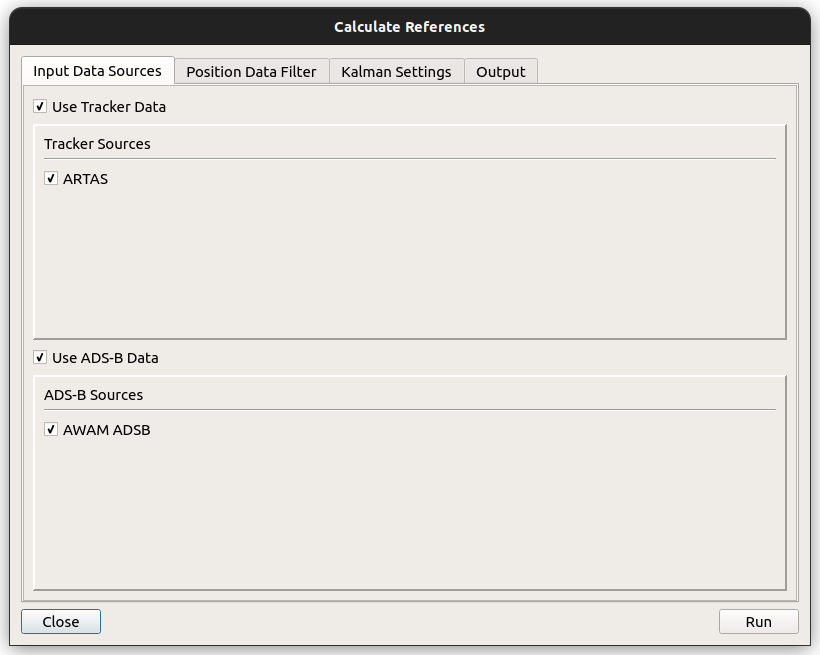
\includegraphics[width=14cm]{figures/ui_task_references_dialog.png}
%     \caption{Calculate References Task - Configuration Dialog}
% \end{figure}

It consists of several configuration tabs:

\begin{itemize}
    \item \textbf{Input Data Sources}: Configuration of data sources to use for reference computation.
    \item \textbf{Position Data Filter}: Filtering options for excluding certain target reports from reference computation.
    \item \textbf{Kalman Settings}: Configuration of the Kalman reconstructor.
    \item \textbf{Output}: Configuration of the generated data source. \\
\end{itemize}

These configuration tabs will be described in more detail below.

\subsubsection{Input Data Sources}

% \begin{figure}[H]
%     \center
%       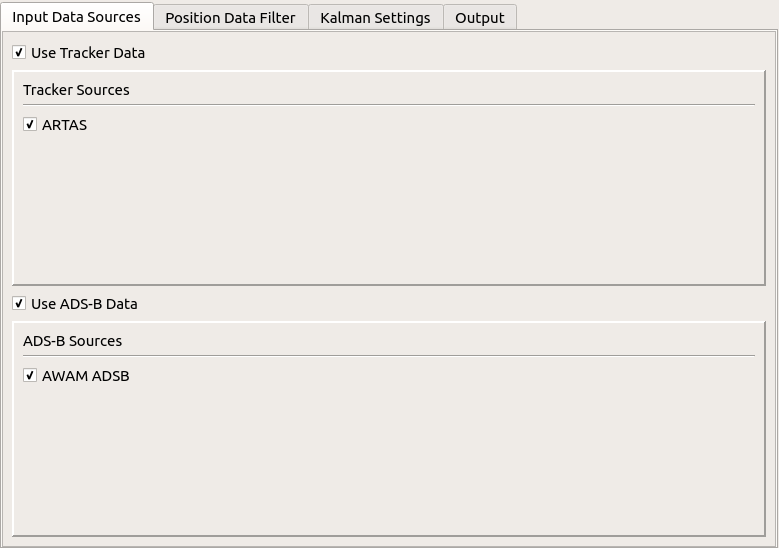
\includegraphics[frame,width=14cm]{figures/ui_task_references_tab_inputds.png}
%     \caption{Calculate References Task - Input Data Sources Tab}
% \end{figure}

In this dialog the data sources which are incorporated into reference trajectory estimation can be configured.
There exists a checkbox for each possible DSType and then a nested list of checkboxes for individual data sources. \\

\textbf{Note}: At least one data source has to be selected in order to run reference computation.

\subsubsection{Position Data Filter}

% \begin{figure}[H]
%     \center
%       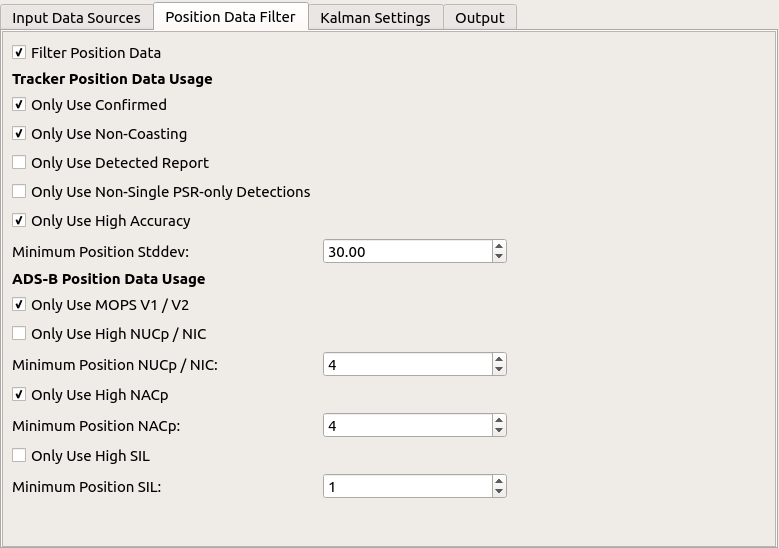
\includegraphics[frame,width=14cm]{figures/ui_task_references_tab_filter.png}
%     \caption{Calculate References Task - Position Data Filter Tab}
% \end{figure}

In this dialog various filters can be enabled in order to remove certain target reports from reference computation. 
The following tables describe the existing options.

\begin{table}[H]
    \center
    \begin{tabularx}{\textwidth}{ | l | l | X |}
        \hline
        \textbf{Parameter} & \textbf{Default} & \textbf{Description} \\ \hline
        Filter Position Data & enabled & Enables/disables filtering of position data \\ \hline
    \end{tabularx}
\end{table}

\textbf{Note}: All other options will be ignored if this option is disabled. \\

\textit{Tracker Position Data Usage}:
\begin{table}[H]
    \center
    \begin{tabularx}{\textwidth}{ | l | l | X |}
        \hline
        \textbf{Parameter} & \textbf{Default} & \textbf{Description} \\ \hline
        Only Use Confirmed & enabled & Use only non-tentative track updates \\ \hline
        Only Use Non-Coasting & enabled & Use only non-coasting track updates \\ \hline
        Only Use Detected Report & disabled & Use only non-zero Detection Type track updates \\ \hline
        Only Use Non-Single PSR-only Detections & disabled & Use no mono PSR-only track updates \\ \hline
        Only Use High Accuracy & enabled & Use only track updates with Std.Dev. smaller than threshold \\ \hline
        Minimum Position Stddev [m] & 30 & Std.Dev. threshold \\ \hline
    \end{tabularx}
\end{table}

\textit{ADS-B Position Data Usage}:
\begin{table}[H]
    \center
    \begin{tabularx}{\textwidth}{ | l | l | X |}
        \hline
        \textbf{Parameter} & \textbf{Default} & \textbf{Description} \\ \hline
        Only Use MOPS V1 / V2 & enabled & Use only MOPS V1 and V2 ADS-B data \\ \hline
        Only Use High NUCp / NIC & disabled & Use only ADS-B data larger than NUCp / NIC threshold \\ \hline
        Minimum Position NUCp / NIC & 4 &  NUCp / NIC threshold \\ \hline
        Only Use High NACp & enabled & Use only ADS-B data larger than NACp threshold \\ \hline
        Minimum Position NACp & 4 & NACp threshold \\ \hline
        Only Use High SIL & disabled & Use only ADS-B data larger than SIL threshold \\ \hline
        Minimum Position SIL & 1 & SIL threshold \\ \hline
    \end{tabularx}
\end{table}

\subsubsection*{Kalman Settings}

% \begin{figure}[H]
%     \center
%       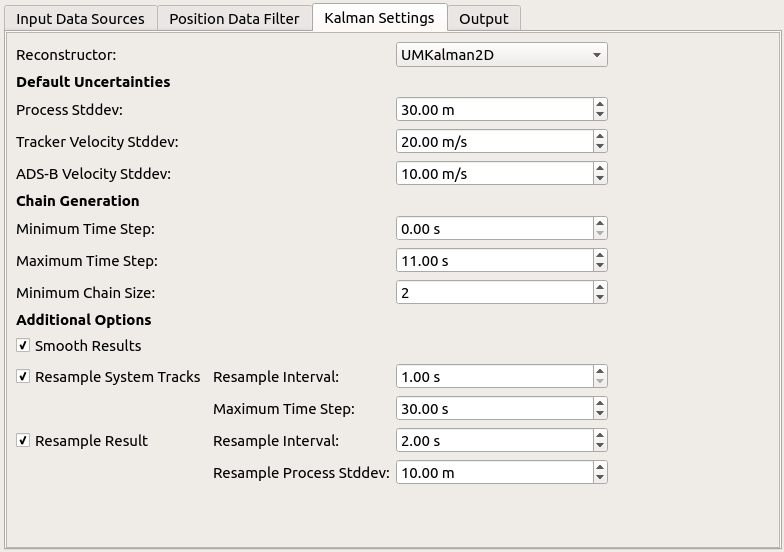
\includegraphics[frame,width=14cm]{figures/ui_task_references_tab_kalman.png}
%     \caption{Calculate References Task - Kalman Settings Tab}
% \end{figure}

In this dialog the used reference trajectory reconstructor can be chosen and configured.
The following tables describe the existing options.

\begin{table}[H]
    \center
    \begin{tabularx}{\textwidth}{ | l | l | X |}
        \hline
        \textbf{Parameter} & \textbf{Default} & \textbf{Description} \\ \hline
        Reconstructor & UMKalman2D & Reconstructor type used for reference computation \\ \hline
    \end{tabularx}
\end{table}

The currently implemented reconstructors are based on the well-known Kalman filter and its various variants.
Currently the following 'flavours' are implemented. \\

\begin{itemize}
    \item \textbf{Uniform Motion Kalman (UMKalman2D)}: 
        Classic Kalman filter assuming a constant velocity between consecutive measurements
    \item \textbf{Accelerated Motion Kalman (AMKalman2D)}: 
        Unscented Kalman filter assuming constant acceleration between consecutive measurements \\
\end{itemize}

\textit{Default Uncertainties}: Parameters related to the uncertainties used in the Kalman filter, in addition to those provided 
by the input data.
\begin{table}[H]
    \center
    \begin{tabularx}{\textwidth}{ | l | l | l | X |}
        \hline
        \textbf{Parameter} & \textbf{Default} & \textbf{Unit} & \textbf{Description} \\ \hline
        %Measurement Stddev & 30 & m & Default standard deviation for added measurements \\ \hline
        %Measurement Stddev (high) & 1000 & m & Default high standard deviation for added measurements, 
        %    used if important data is not provided by the data base (e.g. velocity) \\ \hline
        Process Stddev & 30 & m & Process noise standard deviation of the modelled Kalman process \\ \hline
        Tracker Velocity Stddev & 50 & m & Default standard deviation for tracker velocities, 
            used if not provided by the data \\ \hline
        %Tracker Acceleration Stddev & 50 & m & Default standard deviation for tracker accelerations,
        %    used if not provided by the data \\ \hline
        ADS-B Velocity Stddev & 50 & m & Default standard deviation for ADS-B velocities, 
            used if not provided by the data \\ \hline
        %ADS-B Acceleration Stddev & 50 & m & Default standard deviation for ADS-B accelerations, 
        %    used if not provided by the data \\ \hline
    \end{tabularx}
\end{table}

\textbf{Note}: When using the default settings, target reports without position accuracy data are not used for reference position estimation. However, if such filters (in the \textit{Position Data Filter} tab) are disabled, if no position accuracy is provided by the data for a specific target report, a standard value of 100 meters is automatically assumed. \\

Please also note that if an important value such as velocity is not provided by the data, a value of zero with a very high standard deviation of 1000 meters is automatically assumed. \\

\textit{Chain Generation}: Parameters related to criteria causing the reconstructor to reinitialize the Kalman filter, 
resulting in the reference trajectory of a track being split into multiple sub-chains.
\begin{table}[H]
    \center
    \begin{tabularx}{\textwidth}{ | l | l | l | X |}
        \hline
        \textbf{Parameter} & \textbf{Default} & \textbf{Unit} & \textbf{Description} \\ \hline
        Minimum Time Step & 0 & s & Minimum time difference between consecutive measurements (measurements obtaining a 
            lower time difference to their predecessor will be skipped) \\ \hline
        Maximum Time Step & 11 & s & Maximum time difference between consecutive measurements (measurements obtaining a 
            higher time difference to their predecessor will cause the Kalman filter to reset, 
            resulting in a new sub-chain) \\ \hline
        Minimum Chain Size & 2 & & Minimum number of created reference positions in a sub-chain, in order to add the chain 
            to the final result \\ \hline
    \end{tabularx}
\end{table}

\textit{Additional Options}:
\begin{table}[H]
    \center
    \begin{tabularx}{\textwidth}{ | X | l | l | X |}
        \hline
        \textbf{Parameter} & \textbf{Default} & \textbf{Unit} & \textbf{Description} \\ \hline
        Smooth Results & enabled & & Smooth the results of the Kalman filter using a Rauch–Tung–Striebel smoother \\ \hline
        Resample System Tracks & enabled & & Resample input system tracks using cubic spline interpolation \\ \hline
        Resample System Tracks - Resample Interval & 1 & s & Time interval at which system tracks are resampled \\ \hline
        Resample System Tracks - Maximum Time Step & 30 & s & Maximum time difference between consecutive tracker 
            reports in order to resample the segment \\ \hline
        Resample Result & enabled & & Resample the generated reference trajectories by interpolating the final Kalman states
            at a fixed rate \\ \hline
        Resample Result - Resample Interval & 2 & s & Time interval at which the result trajectories are resampled \\ \hline
        Resample Result - Resample Process Stddev & 10 & m & Standard deviation of the Kalman process when interpolating the 
            Kalman states during result resampling \\ \hline
    \end{tabularx}
\end{table}

Resampling of system tracks can be enabled in order to obtain similar sample rates for tracker and ADS-B
data, which reduces a sensor-specific bias of the Kalman filter. Cubic B-splines are used to interpolate the tracker target
reports in a relaxed way. In case a spline segment deviates too strongly from its interval, a linear interpolation is 
used instead. \\

Result resampling can be enabled in order to obtain reference trajectories with a homogeneous sample rate. 
It is carried out by interpolating the Kalman states at fixed time-steps. The accuracy of the resulting samples
follows the Kalman accuracies more closely when interpolating near the endpoints of a segment, and it will decrease
in the middle of a segment. The amount of decrease of accuracy will depend on the time duration of the segment and the used 
process standard deviation (parameter \textit{Resample Process Stddev}).

\subsubsection{Output}

% \begin{figure}[H]
%     \center
%       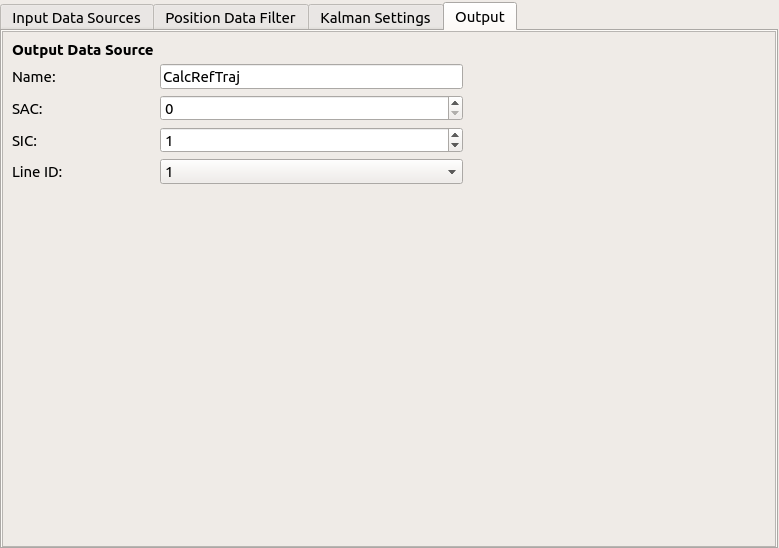
\includegraphics[frame,width=14cm]{figures/ui_task_references_tab_info.png}
%     \caption{Calculate References Task - Output Tab}
% \end{figure}

Here the data source created by reference computation can be configured. 
Reference data will be stored to the database as part of this data source.
The following options are available. \\

\textit{Output Data Source}:
\begin{table}[H]
    \center
    \begin{tabularx}{\textwidth}{ | l | l | X |}
        \hline
        \textbf{Parameter} & \textbf{Default} & \textbf{Description} \\ \hline
        Name & CalcRefTraj & Name of the created data source \\ \hline
        SAC & 0 & SAC of the created data source \\ \hline
        SIC & 1 & SIC of the created data source \\ \hline
        Line ID & 1 & Line ID under which the created data is stored \\ \hline
    \end{tabularx}
\end{table}

Please \textbf{note} that an already existing reference data source is just updated by running the 
reference computation again. This way it is possible to store several reference trajectories to 
different line IDs for the sake of comparison.

\subsubsection{Running The Task}

If configured correctly, the task can be started by clicking the \textit{Run} button.
The current configuration can always be stored without running the task by clicking the \textit{Close} button. 
This can be useful when testing the configuration for using \nameref{sec:ui_proc_calc_references_preview}. \\

When the task is started, the following progress dialog is shown to the user.

% \begin{figure}[H]
%     \center
%       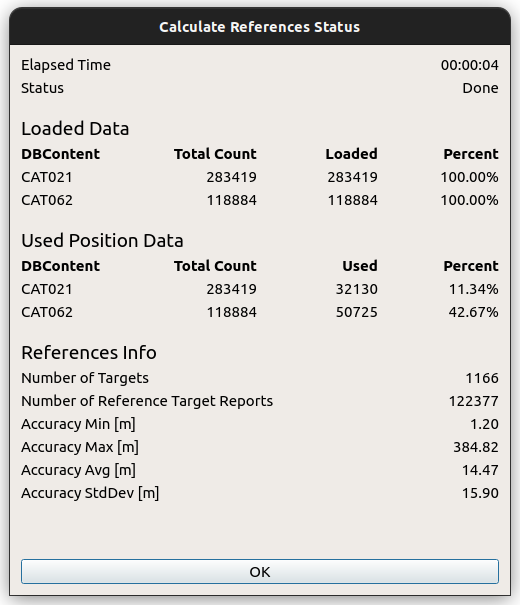
\includegraphics[width=9cm]{figures/ui_task_references_dialog_result.png}
%     \caption{Calculate References Task - Calculate References Status Dialog}
% \end{figure}

First the elapsed time and the current status of the reconstruction process are shown.
Then a few sections give more inside into what happened in the various stages of the process, 
which are described in more detail below.

\paragraph{Loaded Data} This section gives insight into to what ratio data has been loaded from
the database. It shows total and currently loaded data counts, and loading percentage, broken down into
individual DSTypes.

\paragraph{Used Position Data} This section gives insight into to what ratio loaded data has been
included in the reconstruction process after position filtering. 
It shows total data counts, and the amount of data items used for reconstruction in absolute numbers and percentages,
broken down into individual DSTypes.

\paragraph{References Info} This section displays information about the reference computation result.
It shows the number of reference trajectories created, the total number of created target reports, and 
accuracy statistics, which can be used to quantify how well the reconstructor performed.

After finishing, the progress dialog may also display error information. Reference computation can mainly fail in two ways. \\

Badly configured data sources or non-optimal filter settings may result in no data going into the reference computation pipeline.
This will result in the error message \textit{'No input data for reference computation'}. In this case it may help to 
check the included data sources and the chosen filter settings in the reference computation configuration (see above). \\

In case the reconstructor fails to generate any reference data for the included data, the error 
\textit{'No reference data created'} will be shown. A non-optimal Kalman configuration might be the cause for this.

\subsubsection{Reconstruction Preview}
\label{sec:ui_proc_calc_references_preview}

After selecting a desired set of parameters, it can be tiresome to run reference computation for the entire 
set of targets in order to obtain a feedback on the quality of the result. In order to get a faster feedback on the 
chosen parameter set, a \textit{Reconstruction Preview} can be executed for a single chosen track. 
Unlike reference computation for all tracks, the computed reference trajectory will not be written to the database.
Instead it will be visualized in an open Geographic View as an annotation, along with additional intermediate data.
This intermediate data can be especially useful to inspect the various stages of the Kalman process. \\

For this feature, first a set of parameters can be selected in the \textit{Calculate References} dialog, as described above.
Then the current settings are stored by closing the dialog again using the \textit{Close} button on the bottom left. \\

Next, a desired Target can be selected in the \textit{Targets} tab of the main window (see \nameref{sec:ui_targets}).
The reconstruction preview can be started by right-clicking on the selected target and choosing \textit{Reconstruction Preview}.

% \begin{figure}[H]
%     \center
%       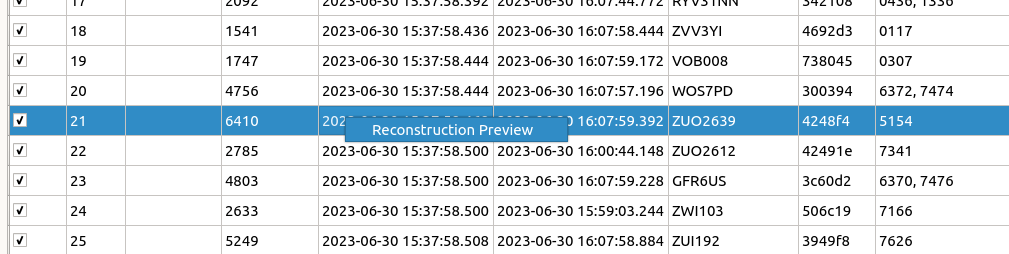
\includegraphics[frame,width=16cm]{figures/ui_task_references_recprev_start.png}
%     \caption{Starting a Reconstruction Preview} 
% \end{figure}

After reconstruction has finished, the results can be inspected in the \textit{Annotations} node of Geographic View's \textit{Layer} tab.

% \begin{figure}[H]
%     \center
%       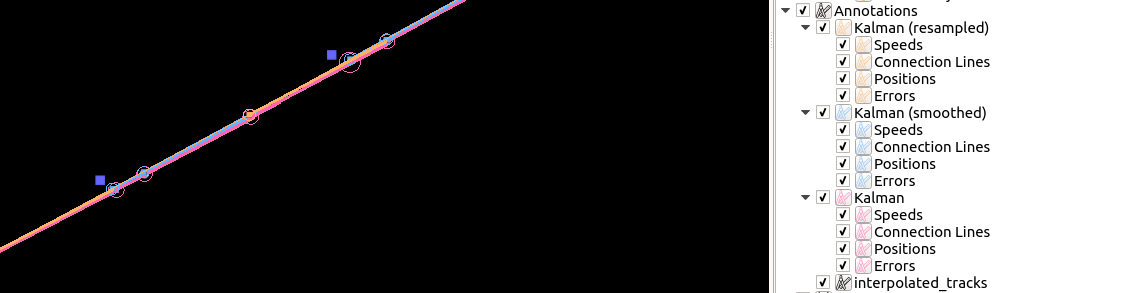
\includegraphics[frame,width=16cm]{figures/ui_task_references_recprev_anno.png}
%     \caption{Reconstruction Preview - Annotations} 
% \end{figure}

Up to three trajectories are shown in different colors, each of them obtaining positions, speed vectors and error ellipses,
and each of them representing different stages of the reconstruction process.

\paragraph{Kalman} Shows the estimates coming directly out of the Kalman filter.
Using this annotation the performance of the Kalman filter can be visually inspected.

% \begin{figure}[H]
%     \center
%       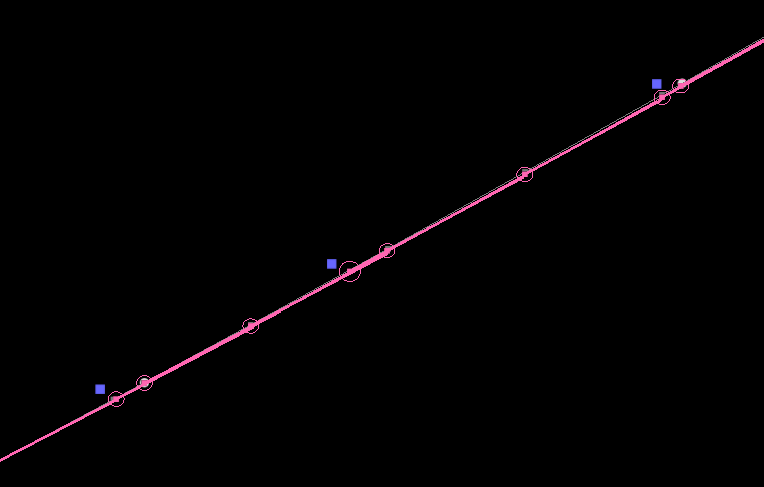
\includegraphics[width=10cm]{figures/ui_task_references_recprev_kalman.png}
%     \caption{Reconstruction Preview - Annotation \textit{Kalman}} 
% \end{figure}

\paragraph{Kalman (smoothed)} Shows the result of the RTS smoother (if smoothing enabled).
Using this annotation the performance of the RTS smoother can be visually inspected.

% \begin{figure}[H]
%     \center
%       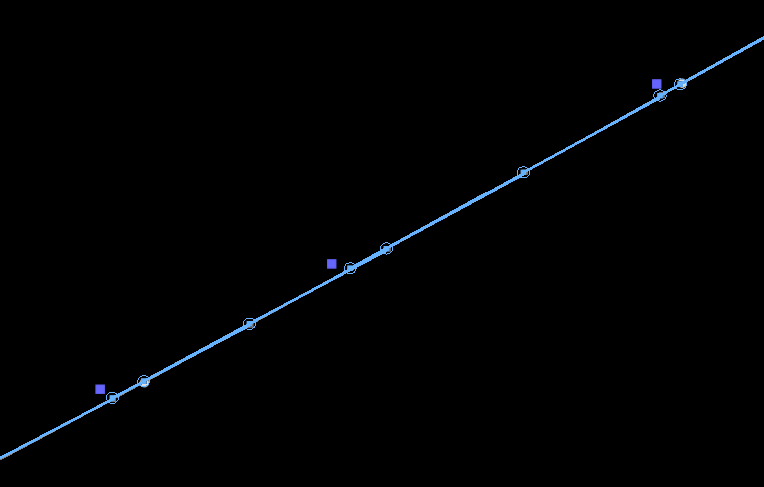
\includegraphics[width=10cm]{figures/ui_task_references_recprev_smoothed.png}
%     \caption{Reconstruction Preview - Annotation \textit{Kalman (smoothed)}} 
% \end{figure}

\paragraph{Kalman (resampled)} Shows the homogeneously resampled Kalman states (if result resampling enabled).
Using this annotation result resampling can be visually inspected.

% \begin{figure}[H]
%     \center
%       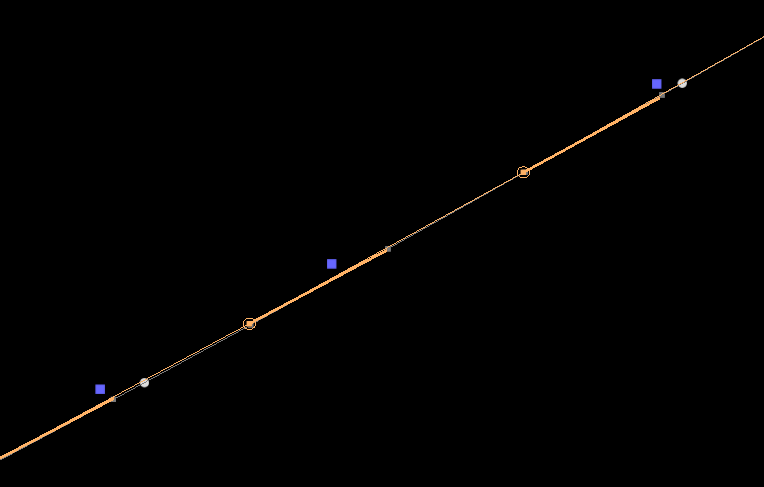
\includegraphics[width=10cm]{figures/ui_task_references_recprev_final.png}
%     \caption{Reconstruction Preview - Annotation \textit{Kalman (resampled)}} 
% \end{figure}

Additionally, an annotation called \textit{Interpolated Tracks} shows the spline-resampled system tracks in grey color,
if system track resampling is enabled.
% 
% \begin{figure}[H]
%     \center
%       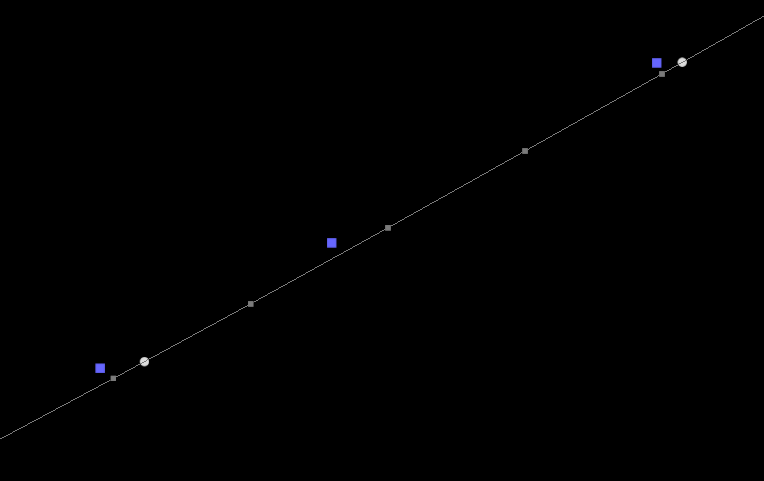
\includegraphics[width=10cm]{figures/ui_task_references_recprev_interp.png}
%     \caption{Reconstruction Preview - Annotation \textit{Interpolated Tracks}} 
% \end{figure}
